\graphicspath{ {./root/1.Inspection/res/} }
\subsection{Final scores}

	\begin{small}

\rowcolors{2}{lightgray}{lightblue}
\begin{longtable}{l r}
	
	\hiderowcolors
	\textbf{Heuristic} & \textbf{Score} \\ \hline  \endhead \\
	\showrowcolors
	

	
	H1. Visibility of system status & 2  \\
	H2. Match between system and the real world & 4  \\
	H3. User control and freedom & 3 \\
	H4. Consistency and standards & 2 \\
	H5. Error prevention & 3 \\
	H6. Recognition rather than recall & 4 \\
	H7. Flexibility and efficiency of use & 3 \\
	H8. Aesthetic and minimalist design & 1 \\
	H9. Help users recognize, diagnose and recover from errors & 5 \\
	H10. Help and documentation & 3 \\
	H11. Information overload & 2 \\
	H12. Consistency of page content structure  & 2 \\
	H13. Contextualized information & 2 \\
	H14. Content organisation (hierarchy) & 4 \\
	H15. Interaction consistency & 1 \\
	H16. Group navigation-1 & 2 \\
	H17. Group navigation-2 & 3 \\
	H18. Structural navigation & 3 \\
	H19. Semantic navigation & 4 \\
	H20. “Landmarks” & 3 \\
	H21. Text lay out & 4 \\
	H22. Interaction placeholders-semiotics & 3 \\
	H23. Interaction placeholders-consistency & 1 \\
	H24. Consistency of visual elements & 3 \\
	H25. Hierarchy-1 & 3 \\
	H26. Hierarchy-2 & 2 \\
	H27. Spatial allocation-1 & 4 \\
	H28. Spatial allocation-2 & 4 \\
	H29. Consistency of page spatial structure & 3 \\
	
	
	
\end{longtable}

\end{small}

\clearpage

\subsection*{Comments}
H1.	In only few pages there are breadcrumbs which can help users to understand where they are, in all other pages there is no way to see the system status.
\newline 
\includegraphics[width=0.6\textwidth]{FinalScores1.jpg}
\newline Another problem is that the section of the menu in which the user is does not highlight, not helping to recognize the system status again.
\newline 
\includegraphics[width=0.7\textwidth]{FinalScores2.jpg}
\newline By clicking on some links, the user is redirected in other websites very similar to the precedent one unless for a little subtitle on the header, this does not help to understand that you are in a different website and may cause confusion.
\newline 
\includegraphics[width=0.8\textwidth]{FinalScores3.jpg}
\newline
\newline H2.	In general, the language used on the website matches the user’s existing knowledge and mental models, making it easy for it to understand the information provided. Also, the icons used on the website represent familiar concepts, facilitating the comprehension.
\newline 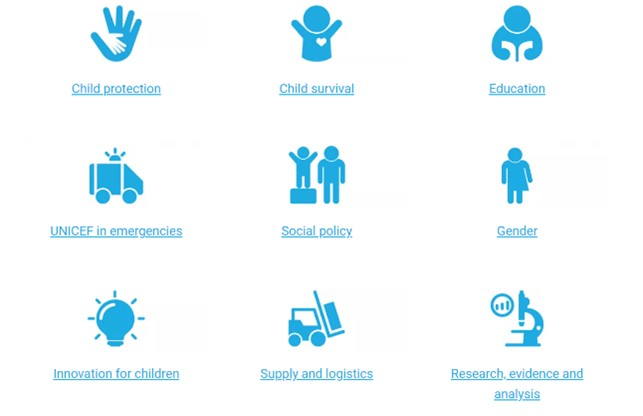
\includegraphics[width=0.5\textwidth]{FinalScores4.jpg}
\newline However, there are instances where the adopted solutions are not so clear, like in the page: \href{https://www.unicef.org/where-we-work}{Where we work | UNICEF}. In fact, the “Browse areas by alphabetical listing” could be done much better with a graphical representation of a map where you could click on the nation.
\newline 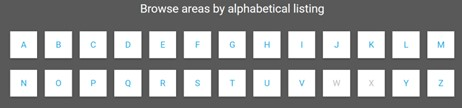
\includegraphics[width=0.8\textwidth]{FinalScores5.jpg}
\newline We also found a Non-functioning button “Join UNICEF” on the page:  \href{https://www.unicef.org/partnerships}{https://www.unicef.org/partnerships} where the communication of the error is not matching good the real world.
\newline
\newline H3.	A good example of the user control implemented on this website is the search engine, where it’s always possible to select the desired filters and search what you want.
\newline 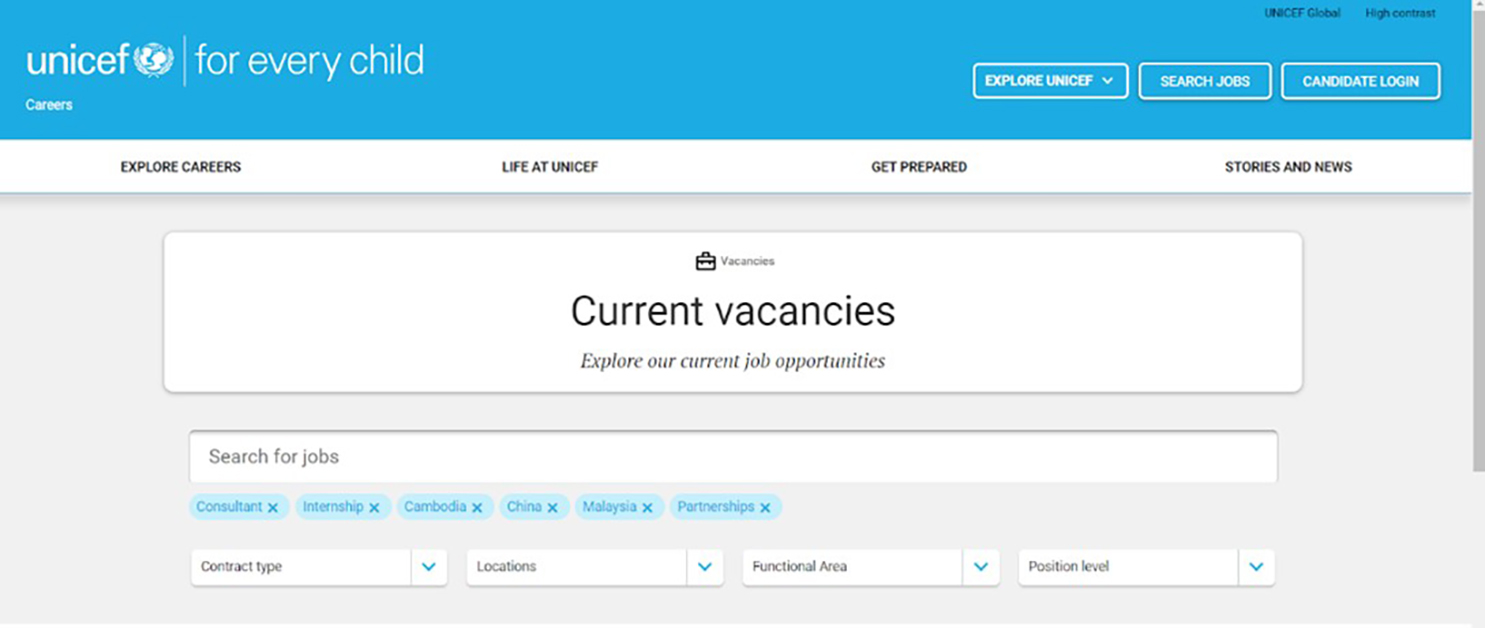
\includegraphics[width=0.8\textwidth]{FinalScores6.jpg}
\newline However, there is a limited sense of freedom: the only page in which the ‘undo’ feature is requested is the donation page, it is implemented but it obliges the user to reinsert all the personal data.
\newline Also, when you try to change page, a big message appears on the screen, giving a not much sense of freedom.
\newline 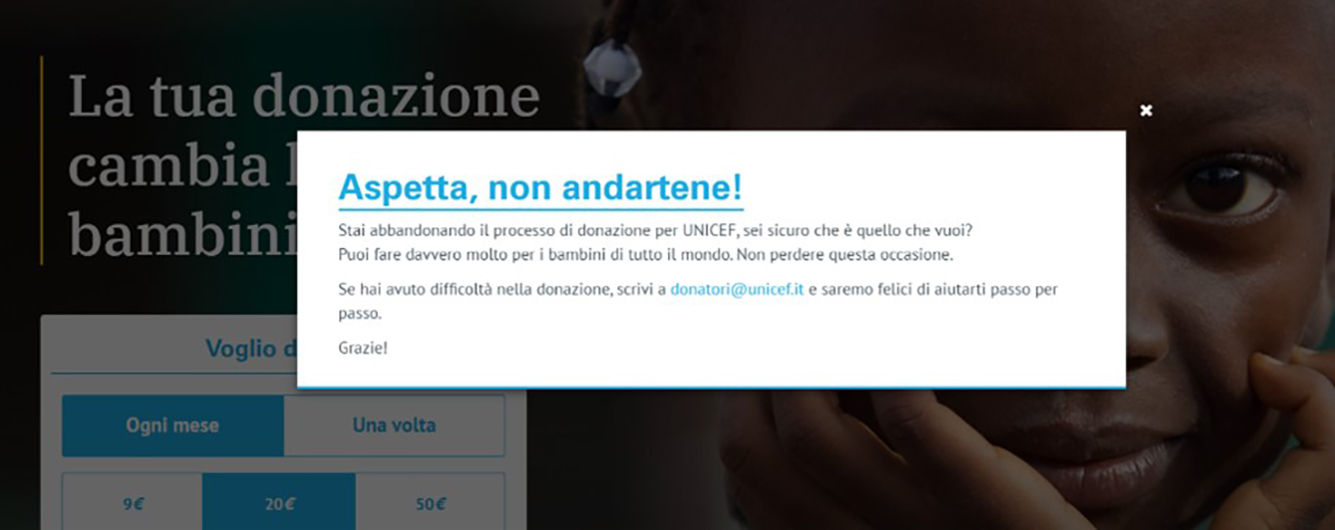
\includegraphics[width=0.7\textwidth]{FinalScores7.jpg}
\newline
\newline H4.	In general, there is a bit of consistency between pages and some standards are respected, but there are also many problems.
\newline The ‘donate’ button is very inconsistent in all the website, and it is red, a colour often used for negative things, which lead at a not respected standard.
\newline 
\includegraphics[width=0.8\textwidth]{FinalScores8.jpg}
\newline There are different and ambiguous meanings, labelling and colours for different cards through the website:
\newline 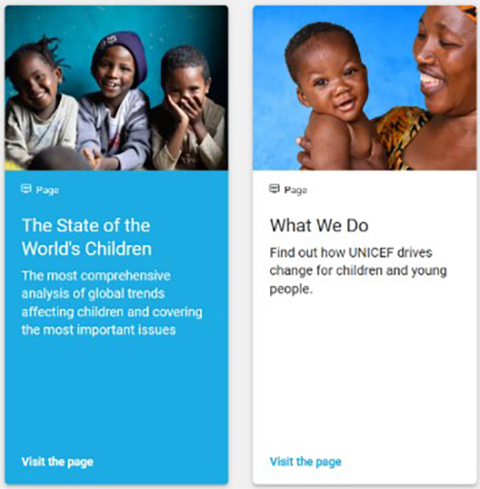
\includegraphics[width=0.5\textwidth]{FinalScores9.jpg}
\newline Two similar icons for two different meanings, and also, they’re not a standard for their meanings:
\newline 
\includegraphics[width=0.5\textwidth]{FinalScores10.jpg}
\newline The donation section on different pages of the section ‘stories’ is not consistent: it’s different in each page, and in some pages it’s even not present.
\newline Another not standard icon we found is in \href{https://www.unicef.org/algeria/agir}{https://www.unicef.org/algeria/agir} , where there is a very strange icon that opens the home page of the website for Algeria.
\newline 
\includegraphics[width=0.7\textwidth]{FinalScores11.jpg}
\newline
\newline H5.	In the donation page, when filling out the form, there is no double check for the user email or a pop up to encourage the user to check again their data for both personal and bank/card.
In this page it is neither showed the minimum quote of donation, which means a missing error prevention.
\newline In the contact page of the section ‘UNICEF data’ (\href {https://data.unicef.org/contact/}{https://data.unicef.org/contact/}) there is a series of fields to fill in, if some of them are incorrectly filled no error message appears, when you click submit all errors appear.
\newline In general, this website is mainly for consulting information and doesn’t offer many interactions with the users that could lead to error-prone situations.
\newline
\newline H6.	Recognition is present when the user uses the searching box.
\newline 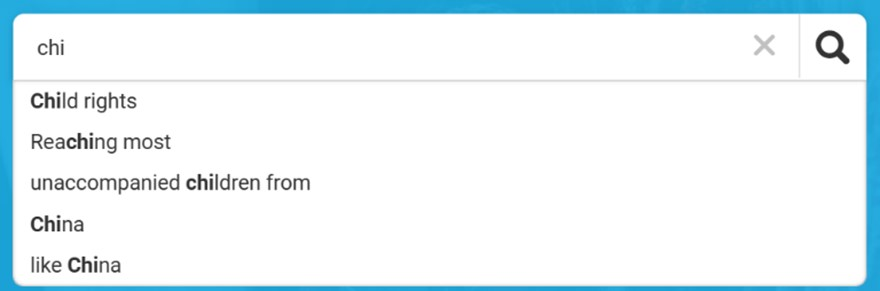
\includegraphics[width=0.6\textwidth]{FinalScores12.jpg}
\newline The drop-down menus also help to recognize, they offer a list of options of the major topics.
\newline In general, all needed information for a specific topic is provided in a single page.
\newline Despite these positive things, there are some pages too nested and too difficult to find even with the search bar (ex. The Skills4Girls page).
\newline
\newline H7.	The website is not too bad for efficiency, in fact the most relevant landmarks are on the page, the problem is that there are only these few web accelerators, and they are less visible.
\newline 
\includegraphics[width=0.5\textwidth]{FinalScores13.jpg}
\newline Regarding flexibility, no customization or personalization is possible across the website, and the interface is difficult to learn, very complex and full of information, making it hard for less experienced users to easily find the information needed. It is neither good for an experienced user, which would like to have a personal section where save articles or frequently visited pages.
\newline
\newline H8.	The interface is not simple or functional, as it is cluttered with many different design elements that often do not follow an established design system. In this way the interface is not supporting the users’ primary goals due to the overload of information.
\newline UNICEF website is complex, due to the need of presenting many different information that support and explain the cause, but its visual design is not focused on the essential and this tragically compromises the user experience.
\newline Some examples are the page \href{https://www.unicef.org/reports/state-worlds-children-2023}{https://www.unicef.org/reports/state-worlds-children-2023} and the not essential quiz in the page \href{https://www.unicef.org/on-my-mind}{OnMyMind: Better mental health for every child | UNICEF} which could have been hidden instead of filling the whole screen. 
\newline 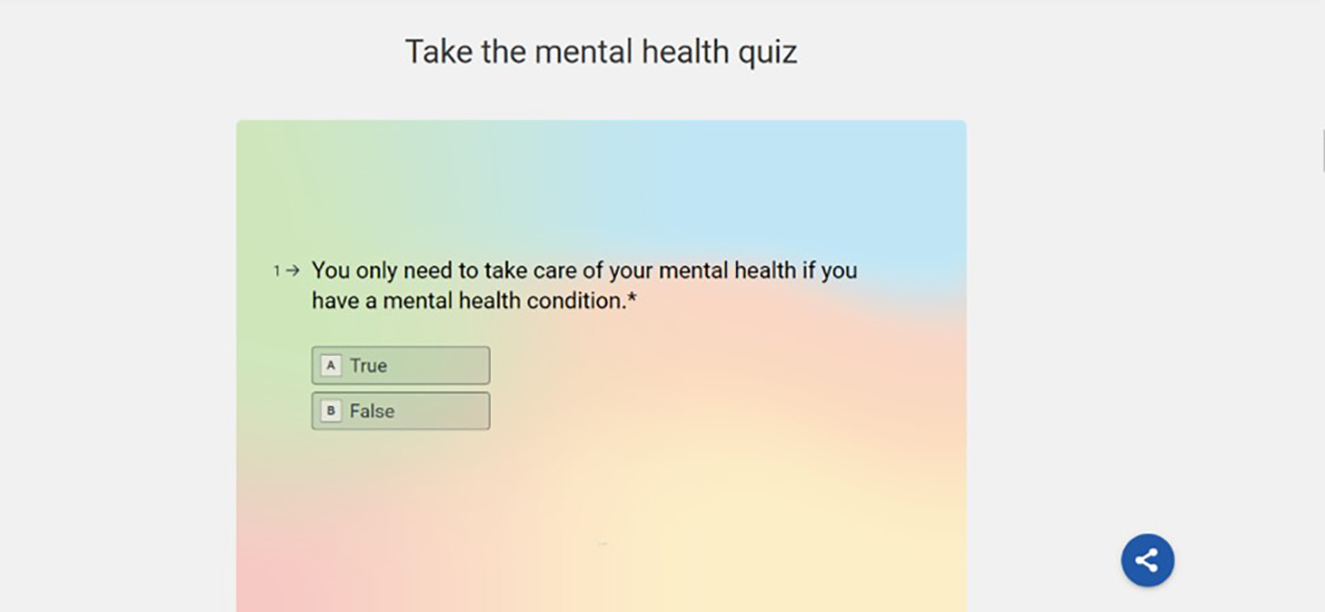
\includegraphics[width=0.7\textwidth]{FinalScores14.jpg}
\newline
\newline H9.	Mistakes when filling forms are correctly highlighted, they are expressed in plain language (no error codes), precisely indicate the problem, and constructively suggest a solution.
\newline 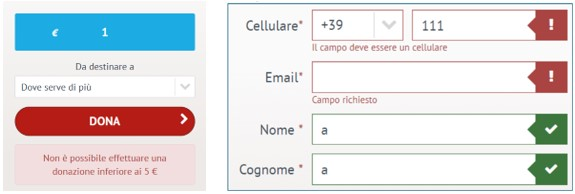
\includegraphics[width=0.9\textwidth]{FinalScores15.jpg}
\newline
\newline H10.	Help and documentation are well provided by the FAQ page and the contact us page, but they are too difficult to find.
\newline
\newline H11.	Really often, in the various pages of the website, there are so many unnecessary information, images, links and other elements, this lack of conciseness creates difficulties in achieving the tasks. A clear example is the page \href{https://www.unicef.org/reports/state-worlds-children-2023}{https://www.unicef.org/reports/state-worlds-children-2023}.
\newline In only few cases information is correctly divided by colours/sections, and some pages are still acceptable, like the home page \href{https://www.unicef.org/}{UNICEF} or the donation page (\href{https://donazioni.unicef.it}{Una donazione per aiutare i bambini - Comitato Italiano per l'UNICEF Fondazione ETS}).
\newline
\newline H12.	In some pages of the same type there is consistency, for example the two pages \href{https://www.unicef.org/gender-equality}{Gender equality | UNICEF} and \href{https://www.unicef.org/health}{Health | UNICEF} have the same style and structure.
\newline However, there are a lot of pages of the same type in which the structure is not the same and which contains different types of elements, this happens, for example, in pages of the section ‘Focus Area’.
\newline Also, in the section ‘stories’ all the pages have a different donation section, creating inconsistency between them.
\newline 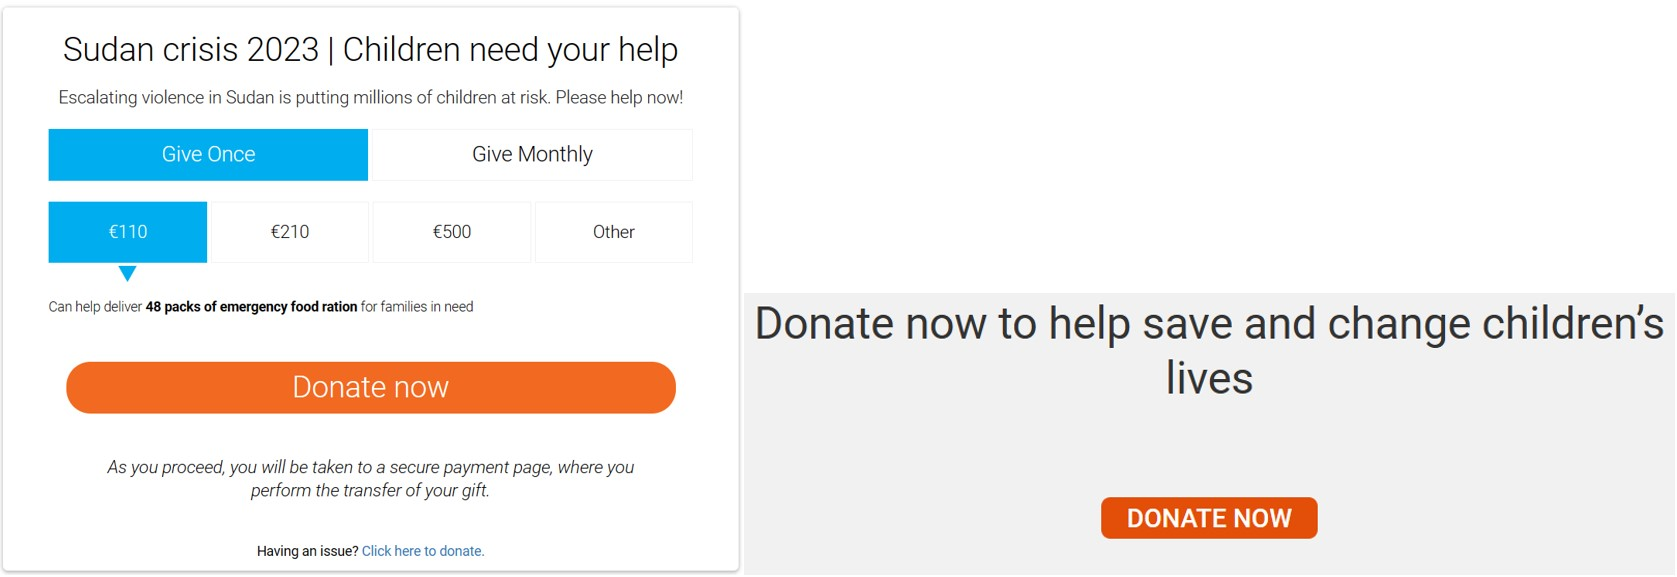
\includegraphics[width=\textwidth]{FinalScores16.jpg}
\newline
\newline H13.	Some elements can help users to understand where they are, for example the title or the image at the top of each page, but it is not enough.
\newline 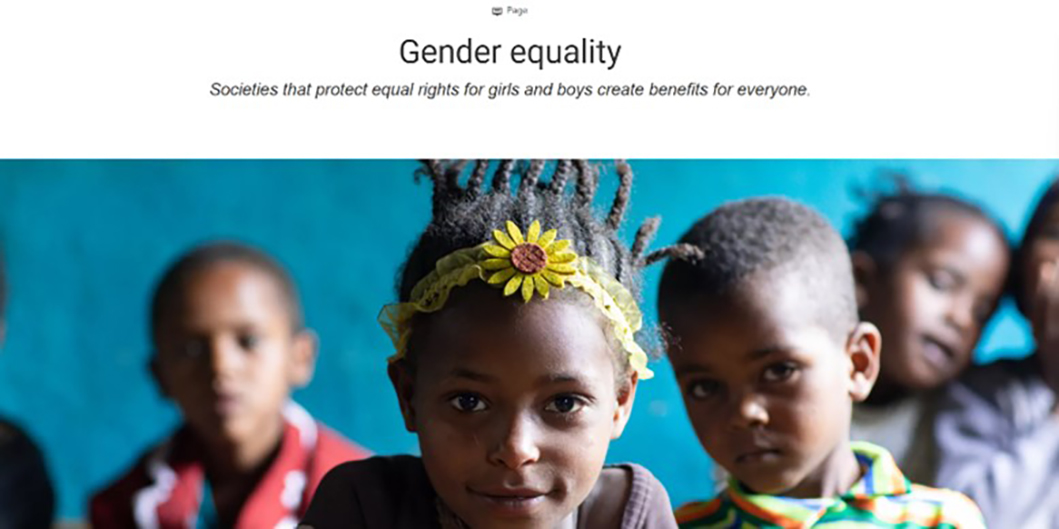
\includegraphics[width=0.7\textwidth]{FinalScores17.jpg}
\newline Breadcrumbs at the top of the pages are not consistent, they are present only in few pages, these elements could help users if they were always present.
\newline Also highlighting the name of the menu in which the user is would help.
\newline
\newline H14.	The content is organized in an understandable manner, even it is not the most intuitive and it can generate a bit of confusion.
\newline The hierarchy is mainly represented by the main 5 section of the menu, the subsections of each of them, and then there are hierarchical relations inside some pages.   
\newline 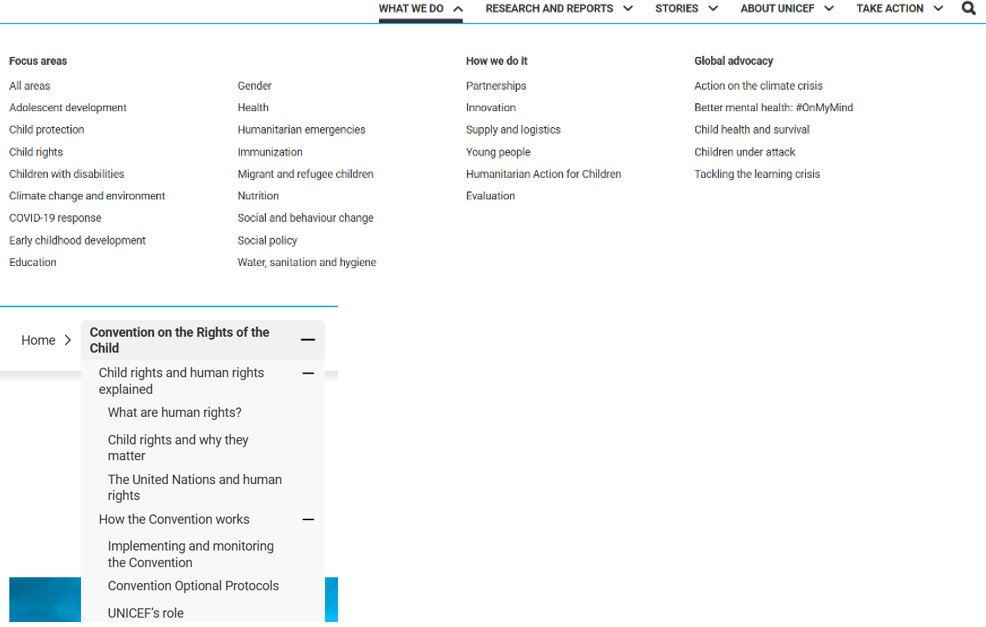
\includegraphics[width=\textwidth]{FinalScores18.jpg}
So, sections and categories are well organized, but sometimes they are redundant in the hierarchy, since they may belong to various sections like \href{https://www.unicef.org/partnerships}{UNICEF partnerships | UNICEF} which belongs both to “Take action” and “What we do”, even though it could have been present in only the first instance. 
\newline A negative aspect is that really often there are some links on the pages which doesn’t really belongs to a precise hierarchy, but they are fundable only in this way.
\newline
\newline H15.	The menu should be always the same, but there are pages in which it is totally different, in fact the two pages \href{https://www.unicef.org/careers/}{UNICEF Careers | UNICEF Careers} and \href{https://www.unicef.org/partnerships}{UNICEF partnerships | UNICEF} have different menus. Even changing the language leads to pages with different menus and different interactions with them (they are no more drop-down menus).
\newline In addition, between pages of the same type, there are different ways to interact, for example  some pages present “Our focus areas”, some not, some presents the navigable index, some not.
\newline 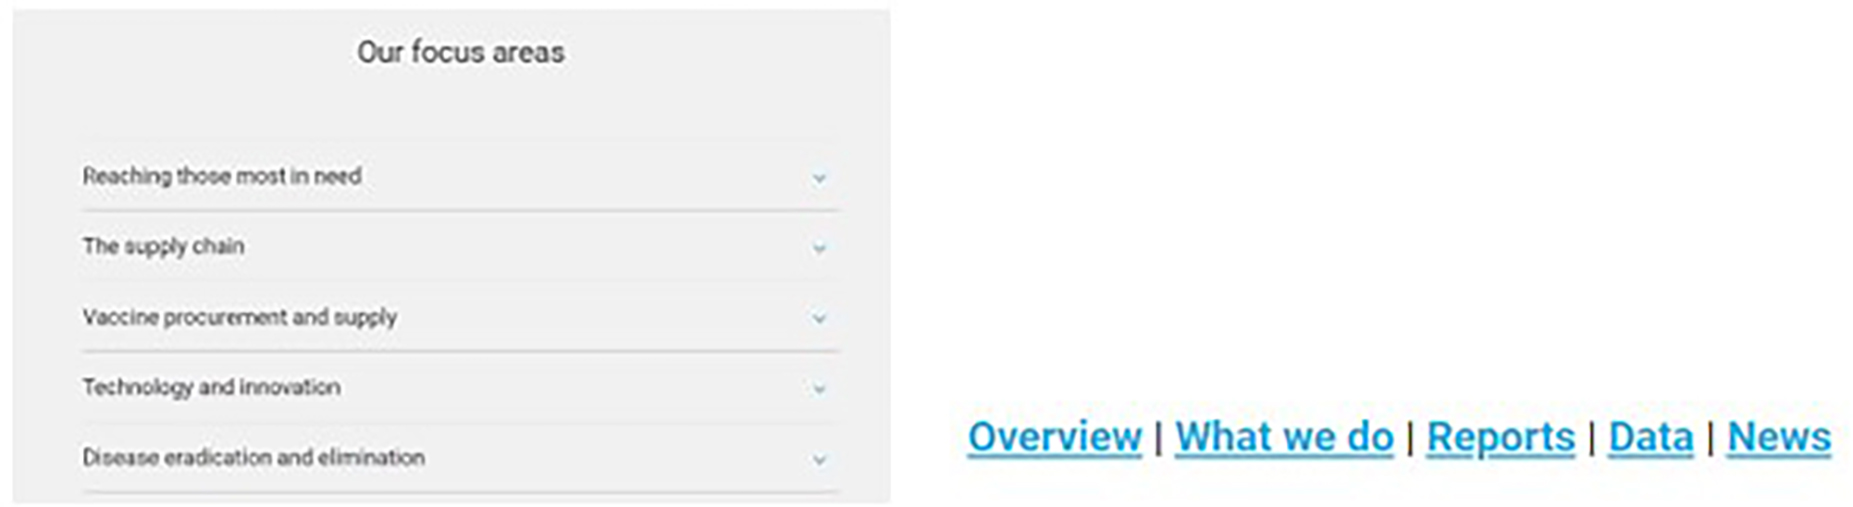
\includegraphics[width=\textwidth]{FinalScores19.jpg}
\newline And again, also the interaction with the donation section of each page is different.
\newline
\newline H16.	When breadcrumbs are present, the navigation in a specific topic is relatively easy, but in most of the website these are not present, and as result it is easy to navigate from the general section to subpages, but not the other way and not even among subpages, for example when from a page you visit a related article it is difficult to go back.
\newline We also noticed that there is impossibility to see articles in chronological order, and in general there is not a real order between articles so there is not the possibility, for example, to go to the next article.
\newline So, the navigation is confusing.
\newline
\newline H17.	The main menu contains a lot of information, but it is quite intuitive and clear, with the section clearly differentiated with consistent names that matches the real world with an appropriate font size. However, there are some inconsistencies like the titles of the menus which are links to some pages, or names being presented differently when opening the page. These discrepancies may create cognitive load. 
\newline In addition, there are some links that lead to different websites and it’s not clear until the user clicks on them, this also create confusion.
\newline 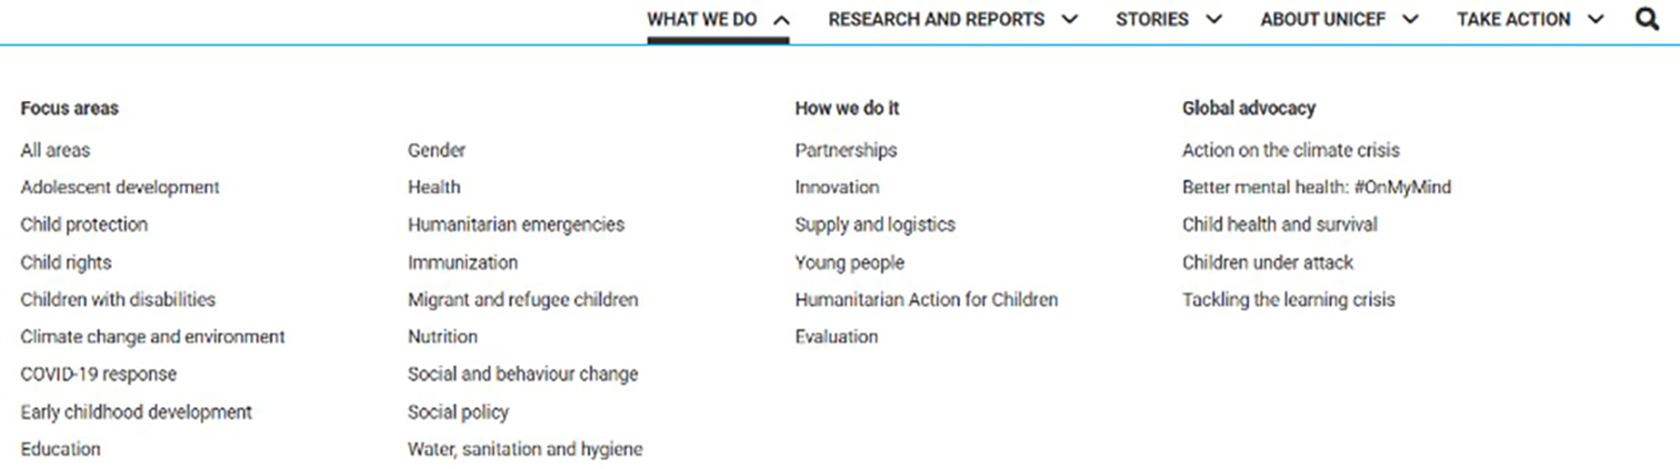
\includegraphics[width=\textwidth]{FinalScores20.jpg}
\newline
\newline H18.	It’s easy enough to navigate among components of a single topic (a single page), but usually, the navigation between a topic and his related articles is quite complex, in fact after opening a link, usually it’s not possible to go back.
\newline A negative aspect of the navigation in a single topic is the hierarchy, which does not help users to understand which part to prioritize: usually similar size and same font for all the elements of a single page.
\newline An example of bad navigation in a page is \href{https://www.unicef.org/reports/state-worlds-children-2023}{https://www.unicef.org/reports/state-worlds-children-2023}, where even background images create confusion.
\newline
\newline H19.	Usually, similar topics are grouped and linked by a new drop-down menu, this makes easy to navigate among related topics in both directions, but this happens only for some pages.
\newline 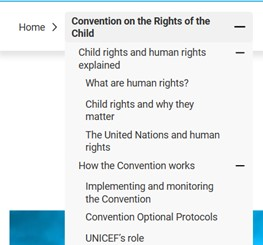
\includegraphics[width=0.4\textwidth]{FinalScores21.jpg}
\newline In some pages there are also sections like ‘related topics’ or ‘find out more’ which help to navigate from a topic to a related one, but not vice-versa.
\newline 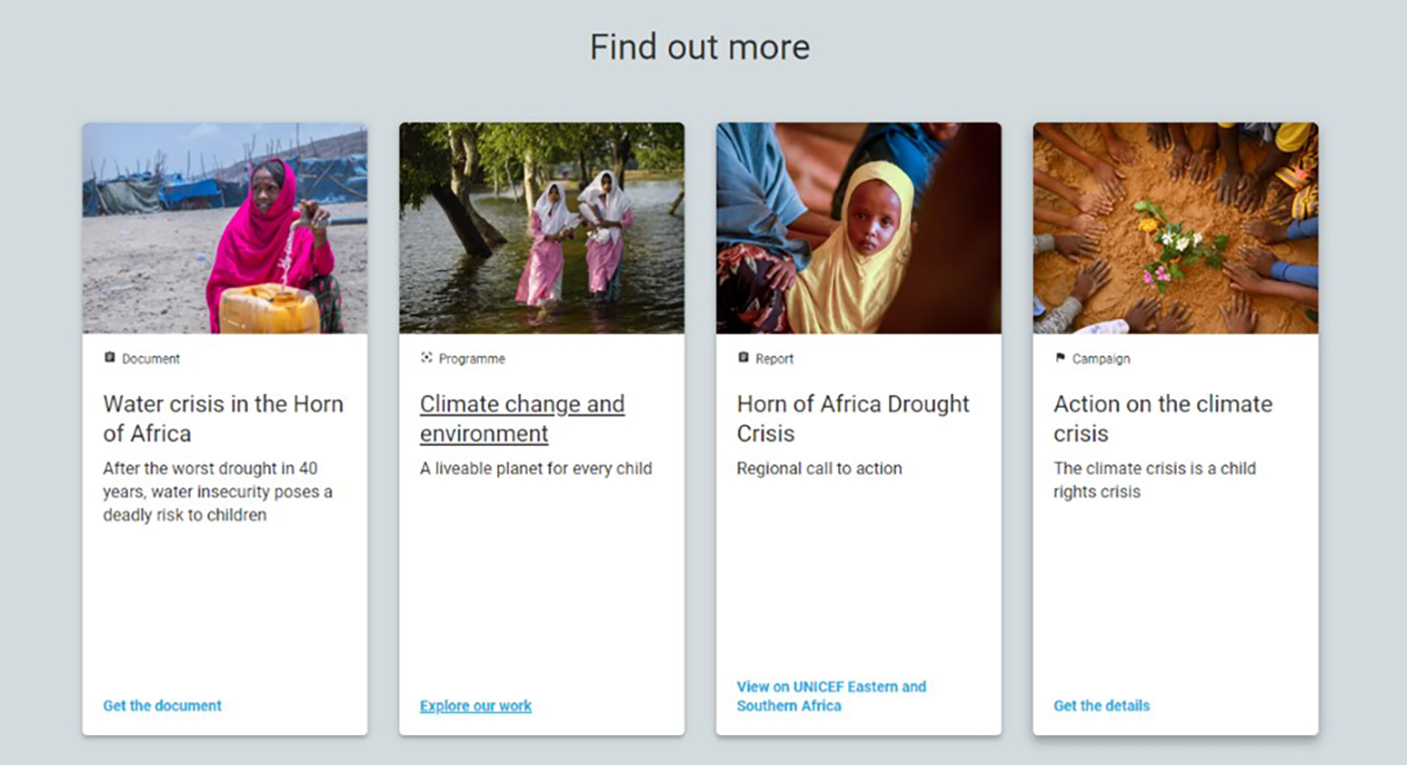
\includegraphics[width=0.7\textwidth]{FinalScores22.jpg}
\newline
\newline H20.	In general landmarks provide a fast access to the main parts of the website, both in the header and in the footer, but most of them are less visible and difficult to find, like the ‘contact us’ in the footer.
\newline There is a problem with the landmark of the home: sometimes happens that the user reaches a different section of the website and the destination of the home landmark change, for example the home landmark of the page \href{https://www.unicef.org/careers/}{UNICEF Careers | UNICEF Careers} does not take to the true home page of the website, but there is a different landmark that is less visible and less intuitive.
\newline 
\includegraphics[width=0.6\textwidth]{FinalScores23.jpg}
\newline Some positive things are the landmark to share an article that is always present in the bottom-right of the screen, and the menu which scrolls down with the user, unfortunately it’s not the same for the logo.
\newline
\newline H21.	In general, the font size is appropriate and the text is readable, there are only few elements which are less visible.
\newline 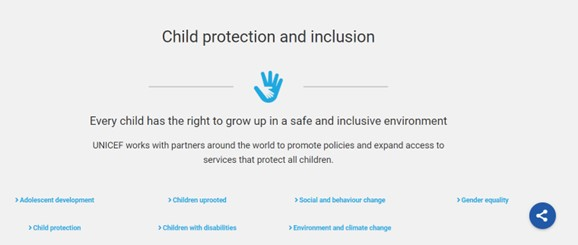
\includegraphics[width=0.8\textwidth]{FinalScores24.jpg}
\newline In addition, the text of the body could be a little smaller to give a better visual hierarchy in the pages.
\newline
\newline H22.	There are many intuitive elements on the website: links are coloured and underlined when overlaying with the mouse; clickable cards have an overlay shadow, as well as textual and primary buttons.
\newline But there are also some elements less intuitive:
\newline -	The drop-down menus are also links.
\newline -	Many other links are not clear where they lead or if they open a new website.
\newline -	The ‘data and insight’ section of some pages contains icons which are clickable links, but they don’t seem links at all.
\newline 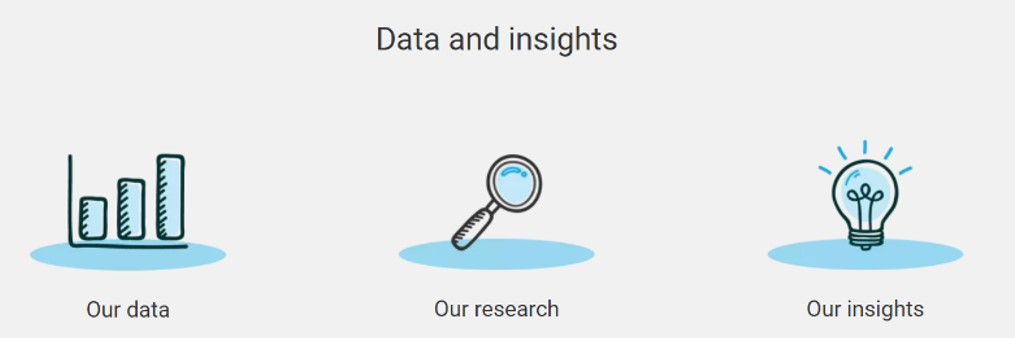
\includegraphics[width=0.6\textwidth]{FinalScores25.jpg}
\newline -	On the page \href{https://www.unicef-irc.org/}{https://www.unicef-irc.org/} there is a functionality to modify the font size which is less intuitive.
\newline 
\includegraphics[width=0.7\textwidth]{FinalScores26.jpg}
\newline
\newline H23.	There are many inconsistent visual elements, the ‘donate’ button is always different and same for the cards.
\newline 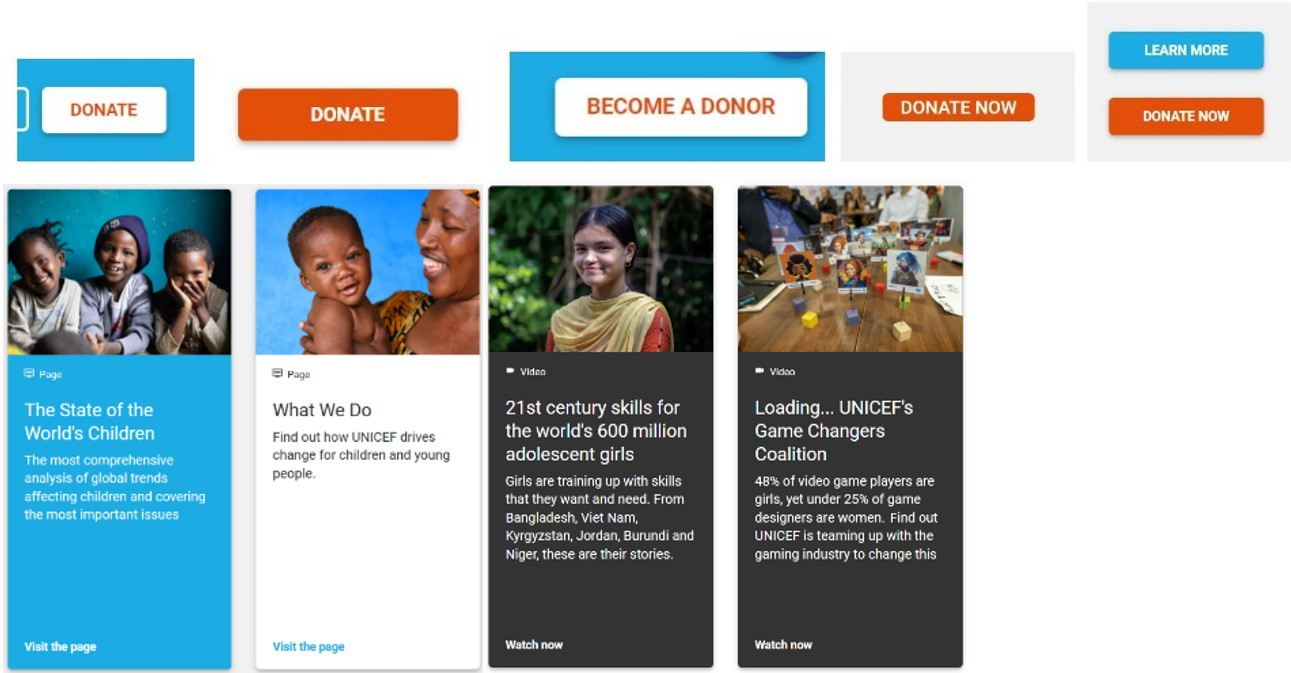
\includegraphics[width=0.8\textwidth]{FinalScores27.jpg}
\newline There is inconsistency in how videos are presented in the page, sometimes are links and sometimes are integrated in the page.
\newline Also reports presents inconsistency because interactions in reports are totally different from other pages interactions.
\newline
\newline H24.	In pages of the same type there is some consistency between visual elements in the sense that they have the same visual properties, but there are also elements which create confusion.
\newline As already mentioned, the inconsistency of the donate buttons and the menus in different pages of the website create confusion in the user, but also cards often have different visual properties: some cards have no images, other are missing of the title or the description.
\newline 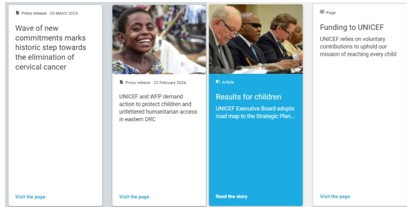
\includegraphics[width=0.7\textwidth]{FinalScores28.jpg}
\newline Resources of different articles have different properties too. In fact, sometimes they are showed with simple links, other times with tables or more complicated links.
\newline 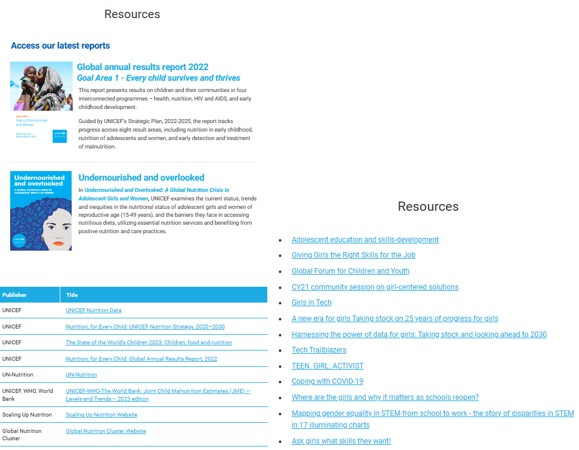
\includegraphics[width=\textwidth]{FinalScores29.jpg}
\newline
\newline H25.	The vertical order in which the elements are in the pages helps to give a sense of hierarchy. On the contrary, the dimensions of various elements through the page are often the same, even the text size is often the same in important elements and in less relevant elements, this does not help to hierarchy.
\newline
\newline H26.	Some important elements have the right relevance in the page, like the logo in the top-left, and the donate button which is always visible and in the top of the page.
\newline But all the visual elements occupy almost the same space in the page, even elements with a lot of different relevance, giving not some sense of hierarchy between them.
\newline The positioning and dimensioning of cards through the pages give a lot of confusion in the user to understand which are the most important elements and which are not.
\newline Also the text in different visual elements is often the same, but the relevance of them should be different.
\newline
\newline H27.	Generally, semantically related elements are close to each other.
\newline 
\includegraphics[width=0.4\textwidth]{FinalScores30.jpg}
\newline Only few elements are bad positioned, one example is the ‘contact us’ landmark which is expected to be in the drop-down menu ‘about UNICEF’ because they are semantically related, but it is in the footer, so distant.
\newline
\newline H28.	Semantically distant elements are usually divided with section of different colours (grey), but the body font size makes it hard to distinguish between each section. 
\newline 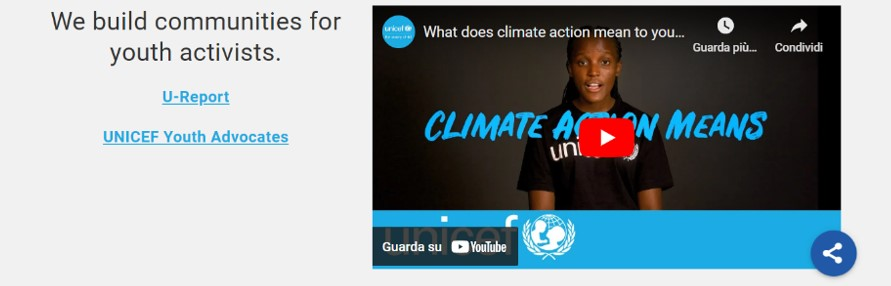
\includegraphics[width=0.7\textwidth]{FinalScores31.jpg}
\newline The ‘press centre’ button should not be at the top-right of the page because it’s not related to the header and to the donate button, maybe it should be in the white bar with the drop-down menus.
\newline 
\includegraphics[width=\textwidth]{FinalScores32.jpg}
\newline
\newline H29.	In general, pages of the same type have similar structures: title, sections and images often in similar positions. There are some instances of similar pages where structures are different, for example in pages of the section ‘stories’ there are different elements and different sections.
\newline It’s simply to see the differences between the pages \href{https://www.unicef.org/emergencies/war-ukraine-pose-immediate-threat-children}{War in Ukraine: Support for children and families | UNICEF} and \href{https://www.unicef.org/emergencies/syrian-crisis}{Syrian crisis | UNICEF}.




















